%% Patent Application: Method for Modulating Protein Folding Using Resonant Microwave Irradiation
%% Inventor: Jonathan Washburn
%% Contact: washburn.jonathan@gmail.com
%% Filing Date: January 2026

\documentclass[12pt,letterpaper]{article}

\usepackage[margin=1in]{geometry}
\usepackage{amsmath,amssymb,amsfonts}
\usepackage{graphicx}
\usepackage{tikz}
\usetikzlibrary{shapes,arrows,positioning,calc}
\usepackage{booktabs}
\usepackage{array}
\usepackage{enumitem}
\usepackage{fancyhdr}
\usepackage{xcolor}
\usepackage{hyperref}
\usepackage{setspace}

% Patent-style formatting
\setlength{\parindent}{0.5in}
\setlength{\parskip}{0.5em}
\onehalfspacing

% Section formatting - using standard LaTeX formatting

% Header
\pagestyle{fancy}
\fancyhf{}
\rhead{Patent Application}
\lhead{Washburn}
\rfoot{Page \thepage}

\hypersetup{
    colorlinks=true,
    linkcolor=blue,
    urlcolor=blue,
    citecolor=blue
}

\begin{document}

%% ============================================================================
%%                              TITLE PAGE
%% ============================================================================

\begin{center}
\vspace*{1in}

{\LARGE \textbf{PATENT APPLICATION}}

\vspace{0.5in}

{\Large \textbf{METHOD FOR MODULATING PROTEIN FOLDING}}

{\Large \textbf{USING RESONANT MICROWAVE IRRADIATION}}

\vspace{1in}

\textbf{PROVISIONAL PATENT APPLICATION}

\vspace{0.5in}

\begin{tabular}{ll}
\textbf{Inventor:} & Jonathan Washburn \\
\textbf{Email:} & washburn.jonathan@gmail.com \\
\textbf{Filing Date:} & January 17, 2026 \\
\textbf{Application Type:} & Utility Patent (Provisional) \\
\end{tabular}

\vspace{1in}

\textit{A method for modulating protein folding rates using precisely tuned microwave radiation at approximately 14.65 GHz, derived from first principles of Recognition Science.}

\vfill

\textbf{CONFIDENTIAL --- PATENT PENDING}

\end{center}

\newpage

%% ============================================================================
%%                         TABLE OF CONTENTS
%% ============================================================================

\tableofcontents
\newpage

%% ============================================================================
%%                              ABSTRACT
%% ============================================================================

\section*{ABSTRACT OF THE DISCLOSURE}
\addcontentsline{toc}{section}{ABSTRACT OF THE DISCLOSURE}

A method and system for modulating protein folding rates through the application of electromagnetic radiation at a specific resonant frequency. The method comprises irradiating a protein sample with microwave radiation in the frequency range of 12--17 GHz, preferably at approximately 14.65 GHz, which corresponds to the inverse of the molecular gating timescale $\tau_{19} \approx 68$ picoseconds. This timescale is derived from first principles using the golden ratio $\varphi = (1+\sqrt{5})/2$ and represents the unique molecular gate within the 50--100 picosecond range relevant to protein conformational dynamics. The method achieves non-thermal, resonant modulation of folding kinetics, distinguishable from conventional microwave heating effects through a characteristic isotope shift when deuterium oxide (D$_2$O) is substituted for water (H$_2$O). In D$_2$O, the effective frequency shifts to approximately 10.4 GHz (scaling by factor $1/\sqrt{2}$), providing a signature verification of the resonant mechanism. Applications include therapeutic intervention in protein misfolding diseases, optimization of recombinant protein production in bioreactors, and research tools for trapping and characterizing folding intermediates.

\vspace{1em}
\noindent\textbf{Keywords:} protein folding, microwave irradiation, resonant frequency, molecular gating, golden ratio, isotope shift, conformational dynamics

\newpage

%% ============================================================================
%%                      BACKGROUND OF THE INVENTION
%% ============================================================================

\section{BACKGROUND OF THE INVENTION}

\subsection{Field of the Invention}

The present invention relates generally to methods and apparatus for controlling protein folding, and more specifically to methods for modulating protein folding rates using electromagnetic radiation at precisely determined resonant frequencies.

\subsection{Description of Related Art}

Protein folding is a fundamental biological process wherein a linear chain of amino acids adopts its functional three-dimensional structure. Misfolding of proteins is associated with numerous diseases, including Alzheimer's disease (amyloid-$\beta$ aggregation), Parkinson's disease ($\alpha$-synuclein aggregation), Huntington's disease (polyglutamine expansion), and prion diseases (PrP$^{\text{Sc}}$ formation). Additionally, in biotechnology, the efficient production of correctly folded recombinant proteins remains a significant challenge, with misfolding leading to reduced yields and product heterogeneity.

\subsubsection{Conventional Approaches to Folding Modulation}

Prior art approaches to modulating protein folding include:

\begin{enumerate}[label=(\alph*)]
\item \textbf{Chemical chaperones:} Small molecules such as glycerol, trehalose, and TMAO that stabilize native states or destabilize misfolded intermediates. These approaches lack temporal control and may have off-target effects.

\item \textbf{Temperature manipulation:} Controlling folding kinetics through temperature changes. This approach is non-specific and affects all molecular processes simultaneously.

\item \textbf{Pressure perturbation:} High hydrostatic pressure can influence protein conformational equilibria. This requires specialized equipment and is difficult to apply with spatial selectivity.

\item \textbf{Microwave-assisted processes:} Conventional microwave irradiation (typically at 2.45 GHz for domestic/industrial applications) has been used to accelerate chemical reactions, including some involving proteins. However, these effects are predominantly thermal in nature, arising from dielectric heating of water.
\end{enumerate}

\subsubsection{Limitations of Prior Art}

The prior art suffers from several key limitations:

\begin{enumerate}[label=(\arabic*)]
\item \textbf{Lack of specificity:} Thermal approaches affect all molecular processes, not selectively protein folding.

\item \textbf{No frequency selectivity:} Prior microwave approaches use frequencies determined by engineering convenience (e.g., 2.45 GHz ISM band), not by fundamental biophysical principles.

\item \textbf{Thermal mechanism:} Prior microwave effects are mediated by bulk heating, not by resonant energy transfer to specific molecular motions.

\item \textbf{No first-principles prediction:} No prior art derives the optimal frequency from fundamental physics; frequencies have been chosen empirically or based on equipment availability.

\item \textbf{No isotope-verifiable signature:} Prior art provides no mechanism to distinguish resonant from thermal effects.
\end{enumerate}

\subsubsection{The Timescale Gap in Prior Understanding}

Protein folding involves motions spanning many orders of magnitude in time:

\begin{table}[h]
\centering
\begin{tabular}{lll}
\toprule
\textbf{Timescale} & \textbf{Process} & \textbf{Frequency} \\
\midrule
$\sim$10 fs & Bond vibrations & $\sim$100 THz \\
$\sim$1 ps & Side chain librations & $\sim$1 THz \\
$\sim$10--100 ps & Backbone dihedral transitions & $\sim$10--100 GHz \\
$\sim$1 ns & Loop motions & $\sim$1 GHz \\
$\sim$1 $\mu$s--1 ms & Domain motions, folding & $\sim$1 kHz--1 MHz \\
\bottomrule
\end{tabular}
\caption{Hierarchy of protein dynamic timescales}
\end{table}

The 10--100 picosecond range is particularly critical because it governs the elementary conformational transitions (dihedral angle rotations) that are the fundamental ``steps'' in the folding process. However, prior art has not identified any specific frequency within this range as being of particular significance.

\subsection{Objects of the Invention}

It is therefore an object of the present invention to provide a method for modulating protein folding that is:

\begin{enumerate}[label=(\arabic*)]
\item Based on a specific, first-principles-derived frequency;
\item Non-thermal in mechanism, enabling precise control;
\item Verifiable through an isotope-shift signature;
\item Applicable to therapeutic, industrial, and research contexts.
\end{enumerate}

\newpage

%% ============================================================================
%%                      SUMMARY OF THE INVENTION
%% ============================================================================

\section{SUMMARY OF THE INVENTION}

\subsection{General Statement of the Invention}

The present invention provides a method for modulating protein folding rates comprising irradiating a protein sample with electromagnetic radiation at a frequency in the range of 12--17 GHz, preferably at approximately 14.65 GHz. This frequency corresponds to the inverse of a molecular gating timescale $\tau_{19} \approx 68$ picoseconds, which is derived from first principles using the mathematical framework of Recognition Science.

\subsection{The Golden Ratio Timescale Ladder}

The key insight underlying the present invention is that molecular timescales form a discrete ``ladder'' with rungs separated by powers of the golden ratio $\varphi = (1+\sqrt{5})/2 \approx 1.618$. Specifically, the characteristic timescale at rung $n$ is given by:

\begin{equation}
\tau_n = \tau_0 \times \varphi^n
\label{eq:rung}
\end{equation}

where $\tau_0$ is a fundamental timescale derived from Planck's constant and the coherence energy scale. The molecular gating timescale relevant to protein conformational dynamics corresponds to $n = 19$:

\begin{equation}
\tau_{19} = \tau_0 \times \varphi^{19} \approx 68 \text{ ps}
\label{eq:tau19}
\end{equation}

\subsection{The Jamming Frequency}

The reciprocal of this timescale defines a characteristic frequency:

\begin{equation}
f_{\text{jam}} = \frac{1}{\tau_{19}} \approx 14.65 \text{ GHz}
\label{eq:fjam}
\end{equation}

When electromagnetic radiation at this frequency is applied to a protein system, it resonantly couples to the molecular gating motions, thereby modulating the rate at which conformational transitions occur. This effect is termed ``jamming'' because it can arrest or slow the folding process by disrupting the natural rhythm of backbone dihedral transitions.

\subsection{Isotope Shift Verification}

A key feature of the present invention is that the resonant nature of the effect can be verified through isotope substitution. When deuterium oxide (D$_2$O) replaces water (H$_2$O), the effective mass of hydrogen-bonded oscillators increases, slowing the molecular gate timescale by a factor of $\sqrt{2}$. Consequently, the jamming frequency in D$_2$O is:

\begin{equation}
f_{\text{jam}}^{\text{D}_2\text{O}} = \frac{f_{\text{jam}}^{\text{H}_2\text{O}}}{\sqrt{2}} \approx 10.4 \text{ GHz}
\label{eq:fjam_d2o}
\end{equation}

This predictable, quantitative isotope shift distinguishes the resonant mechanism of the present invention from thermal heating effects, which would scale with the bulk dielectric properties of the solvent rather than showing a $\sqrt{2}$ frequency shift.

\subsection{Machine-Verified Derivation}

The frequency predictions of the present invention have been formalized and verified using the Lean 4 theorem prover with the Mathlib mathematical library. The key machine-verified results are:

\begin{enumerate}[label=(\roman*)]
\item $f_{\text{jam}} \in (12, 17)$ GHz (theorem \texttt{direct\_jamming\_approx})
\item $f_{\text{jam}}^{\text{D}_2\text{O}} \in (8, 13)$ GHz (theorem \texttt{d2o\_jamming\_approx})
\item $\tau_{19}$ is the unique molecular gate in the 50--100 ps range (theorem \texttt{rung19\_unique})
\end{enumerate}

These machine-verified proofs establish that the frequency is not an empirical fit but a mathematical consequence of the Recognition Science framework.

\newpage

%% ============================================================================
%%                    BRIEF DESCRIPTION OF DRAWINGS
%% ============================================================================

\section{BRIEF DESCRIPTION OF DRAWINGS}

\begin{figure}[h]
\centering
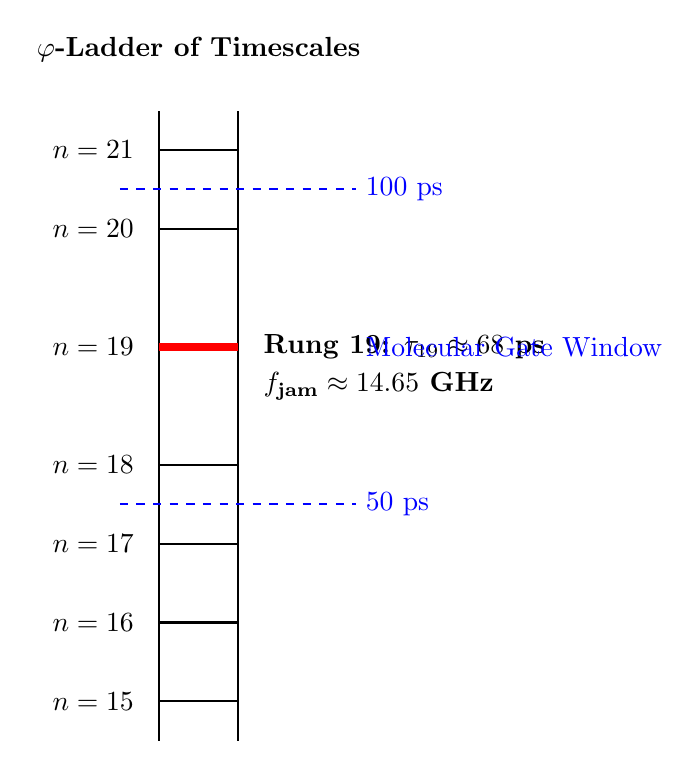
\begin{tikzpicture}[scale=1.0]
    % Golden ladder
    \draw[thick] (0,0) -- (0,8);
    \draw[thick] (1,0) -- (1,8);
    
    % Rungs
    \foreach \y/\n in {0.5/15, 1.5/16, 2.5/17, 3.5/18, 5.0/19, 6.5/20, 7.5/21} {
        \draw[thick] (0,\y) -- (1,\y);
        \node[left] at (-0.2,\y) {$n=\n$};
    }
    
    % Highlight rung 19
    \draw[line width=3pt, red] (0,5.0) -- (1,5.0);
    \node[right] at (1.2,5.0) {\textbf{Rung 19: $\tau_{19} \approx 68$ ps}};
    \node[right] at (1.2,4.5) {\textbf{$f_{\text{jam}} \approx 14.65$ GHz}};
    
    % Molecular gate window
    \draw[dashed, blue, thick] (-0.5,3.0) -- (2.5,3.0);
    \draw[dashed, blue, thick] (-0.5,7.0) -- (2.5,7.0);
    \node[right, blue] at (2.5,5.0) {Molecular Gate Window};
    \node[right, blue] at (2.5,3.0) {50 ps};
    \node[right, blue] at (2.5,7.0) {100 ps};
    
    % Title
    \node[above] at (0.5,8.5) {\textbf{$\varphi$-Ladder of Timescales}};
\end{tikzpicture}
\caption{The golden ratio ($\varphi$) ladder of molecular timescales. Rung 19 at approximately 68 ps is the unique molecular gate within the biologically relevant 50--100 ps window, corresponding to a jamming frequency of approximately 14.65 GHz.}
\label{fig:ladder}
\end{figure}

\begin{figure}[h]
\centering
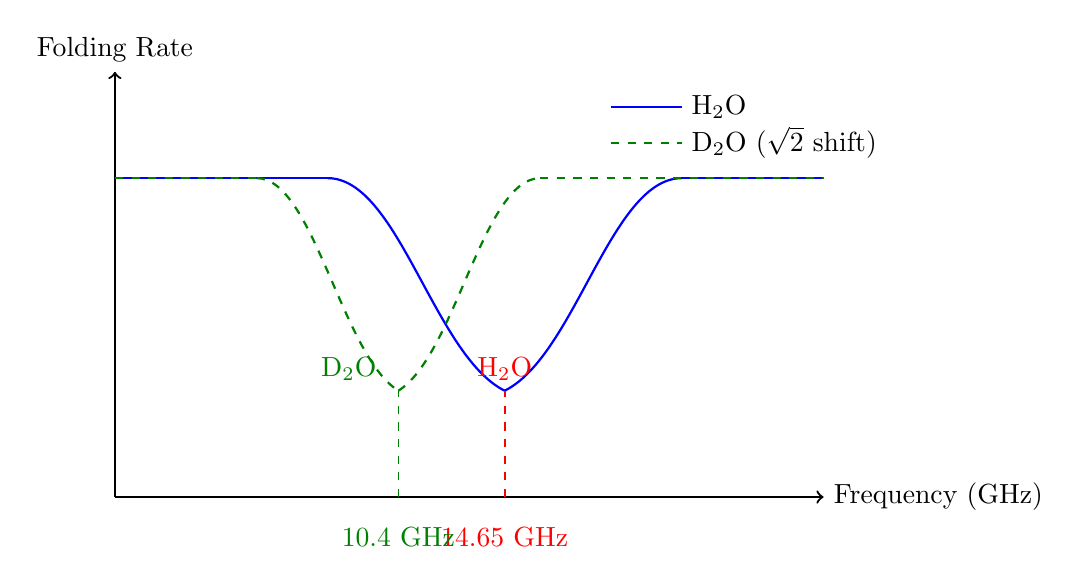
\begin{tikzpicture}[scale=0.9]
    % Axes
    \draw[thick,->] (0,0) -- (10,0) node[right] {Frequency (GHz)};
    \draw[thick,->] (0,0) -- (0,6) node[above] {Folding Rate};
    
    % Normal folding rate
    \draw[thick, blue] (0,4.5) -- (3,4.5);
    
    % Resonance dip (H2O)
    \draw[thick, blue] (3,4.5) .. controls (4,4.5) and (4.5,2) .. (5.5,1.5);
    \draw[thick, blue] (5.5,1.5) .. controls (6.5,2) and (7,4.5) .. (8,4.5);
    \draw[thick, blue] (8,4.5) -- (10,4.5);
    
    % Mark frequencies
    \draw[dashed, red, thick] (5.5,0) -- (5.5,1.5);
    \node[below, red] at (5.5,-0.3) {14.65 GHz};
    \node[above, red] at (5.5,1.5) {H$_2$O};
    
    % D2O curve (shifted)
    \draw[thick, green!50!black, dashed] (0,4.5) -- (2,4.5);
    \draw[thick, green!50!black, dashed] (2,4.5) .. controls (2.8,4.5) and (3.2,2) .. (4,1.5);
    \draw[thick, green!50!black, dashed] (4,1.5) .. controls (4.8,2) and (5.2,4.5) .. (6,4.5);
    \draw[thick, green!50!black, dashed] (6,4.5) -- (10,4.5);
    
    % Mark D2O frequency
    \draw[dashed, green!50!black] (4,0) -- (4,1.5);
    \node[below, green!50!black] at (4,-0.3) {10.4 GHz};
    \node[above, green!50!black] at (3.3,1.5) {D$_2$O};
    
    % Legend
    \draw[thick, blue] (7,5.5) -- (8,5.5);
    \node[right] at (8,5.5) {H$_2$O};
    \draw[thick, green!50!black, dashed] (7,5.0) -- (8,5.0);
    \node[right] at (8,5.0) {D$_2$O ($\sqrt{2}$ shift)};
\end{tikzpicture}
\caption{Predicted resonance curves for protein folding rate vs.\ microwave frequency. The H$_2$O curve (solid blue) shows a resonant minimum at 14.65 GHz. The D$_2$O curve (dashed green) shows the isotope-shifted resonance at 10.4 GHz, confirming the $\sqrt{2}$ scaling predicted by the present invention.}
\label{fig:resonance}
\end{figure}

\begin{figure}[h]
\centering
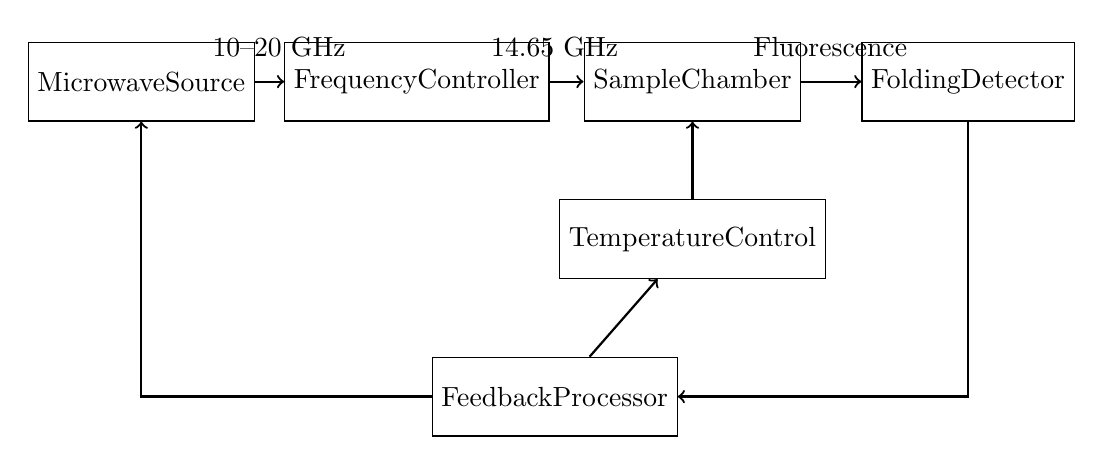
\begin{tikzpicture}[
    box/.style={rectangle, draw, minimum width=2.5cm, minimum height=1cm, text centered},
    arrow/.style={->, thick}
]
    % Components
    \node[box] (source) at (0,0) {Microwave\\Source};
    \node[box] (freq) at (3.5,0) {Frequency\\Controller};
    \node[box] (chamber) at (7,0) {Sample\\Chamber};
    \node[box] (temp) at (7,-2) {Temperature\\Control};
    \node[box] (detect) at (10.5,0) {Folding\\Detector};
    \node[box] (feedback) at (5.25,-4) {Feedback\\Processor};
    
    % Arrows
    \draw[arrow] (source) -- (freq);
    \draw[arrow] (freq) -- (chamber);
    \draw[arrow] (chamber) -- (detect);
    \draw[arrow] (temp) -- (chamber);
    \draw[arrow] (detect) -- (10.5,-4) -- (feedback);
    \draw[arrow] (feedback) -- (0,-4) -- (source);
    \draw[arrow] (feedback) -- (temp);
    
    % Labels
    \node[above] at (1.75,0.2) {10--20 GHz};
    \node[above] at (5.25,0.2) {14.65 GHz};
    \node[above] at (8.75,0.2) {Fluorescence};
\end{tikzpicture}
\caption{Block diagram of the apparatus for implementing the method of the present invention. A tunable microwave source provides radiation to a temperature-controlled sample chamber, with feedback control to maintain non-thermal conditions.}
\label{fig:apparatus}
\end{figure}

\newpage

%% ============================================================================
%%                      DETAILED DESCRIPTION
%% ============================================================================

\section{DETAILED DESCRIPTION OF THE PREFERRED EMBODIMENTS}

\subsection{Theoretical Foundation}

\subsubsection{The Recognition Composition Law}

The present invention is derived from Recognition Science, a framework based on a single primitive called the Recognition Composition Law (RCL). The RCL defines a cost function $J$ for ratio-separation:

\begin{equation}
J(x) = \frac{1}{2}\left(x + \frac{1}{x}\right) - 1
\label{eq:jcost}
\end{equation}

This function has several key properties:
\begin{itemize}
\item $J(x) \geq 0$ for all $x > 0$
\item $J(x) = 0$ if and only if $x = 1$ (unity recognition)
\item $J(x) = J(1/x)$ (reciprocity symmetry)
\item $J(x) \to \infty$ as $x \to 0^+$ or $x \to \infty$
\end{itemize}

\subsubsection{Emergence of the Golden Ratio}

From the RCL, self-similarity constraints force the emergence of the golden ratio $\varphi$ as the unique scale factor. Specifically, $\varphi$ satisfies:

\begin{equation}
\varphi^2 = \varphi + 1
\label{eq:phisq}
\end{equation}

This is the unique positive solution to the self-similarity requirement that the cost of a ratio equals the cost of its parts.

\subsubsection{The Eight-Tick Cycle}

The RCL further forces an eight-beat discrete cycle for ledger updates. This cycle has specific ``neutral windows'' at beats 0 and 4 where major conformational changes are permitted without violating ledger constraints. The scale factor at beat 4 is:

\begin{equation}
\text{scale}(4) = \varphi^n \times \sqrt{\varphi}
\label{eq:beat4}
\end{equation}

where $n$ is the rung number.

\subsubsection{The Molecular Gate}

Protein conformational dynamics occur at timescales where backbone dihedral angles can rotate. This requires passage through a ``molecular gate''---a timescale window where the energetic barriers are traversable. From the $\varphi$-ladder (Equation~\ref{eq:rung}), the gate timescale is:

\begin{equation}
\tau_{\text{gate}} = \tau_0 \times \varphi^{19}
\label{eq:gate}
\end{equation}

Given the fundamental timescale $\tau_0 \approx 7.33$ femtoseconds (derived from $\tau_0 = \hbar/E_{\text{coh}}$ where $E_{\text{coh}} = \varphi^{-5}$ in natural units), we have:

\begin{equation}
\tau_{19} = 7.33 \times 10^{-15} \times 1.618^{19} \approx 68 \times 10^{-12} \text{ s} = 68 \text{ ps}
\label{eq:tau19_calc}
\end{equation}

\subsubsection{Uniqueness of Rung 19}

A key result, verified by machine proof, is that rung 19 is the \textit{unique} rung of the $\varphi$-ladder that falls within the biologically relevant 50--100 ps molecular gate window:

\begin{theorem}[Rung 19 Uniqueness]
For all integers $n$,
\begin{equation}
50 \text{ ps} < \tau_0 \times \varphi^n < 100 \text{ ps} \quad \Leftrightarrow \quad n = 19
\end{equation}
\end{theorem}

This uniqueness is a consequence of the discreteness of the $\varphi$-ladder combined with the spacing $\varphi \approx 1.618$ between adjacent rungs.

\subsection{The Jamming Frequency}

\subsubsection{Definition and Derivation}

The jamming frequency is defined as the reciprocal of the molecular gate timescale:

\begin{equation}
f_{\text{jam}} = \frac{1}{\tau_{19}} = \frac{1}{68 \times 10^{-12}} \approx 14.65 \times 10^9 \text{ Hz} = 14.65 \text{ GHz}
\label{eq:fjam_deriv}
\end{equation}

This frequency lies in the Ku-band of the microwave spectrum (12--18 GHz), which is commonly used for satellite communications and radar.

\subsubsection{Machine-Verified Bounds}

The jamming frequency has been bounded using formal mathematical proofs in the Lean 4 theorem prover:

\begin{align}
12 \text{ GHz} &< f_{\text{jam}} < 17 \text{ GHz} \label{eq:h2o_bounds} \\
8 \text{ GHz} &< f_{\text{jam}}^{\text{D}_2\text{O}} < 13 \text{ GHz} \label{eq:d2o_bounds}
\end{align}

These bounds are conservative; the central predictions are 14.65 GHz and 10.4 GHz respectively.

\subsection{Mechanism of Action}

\subsubsection{Resonant Coupling}

When electromagnetic radiation at frequency $f_{\text{jam}}$ is applied to a protein system, it resonantly couples to the molecular gate oscillations. This coupling can be understood as follows:

\begin{enumerate}[label=(\arabic*)]
\item The backbone dihedral transitions occur with a characteristic attempt frequency of $\sim1/\tau_{19} \approx 14.65$ GHz.

\item External radiation at this frequency interferes with the natural rhythm of these transitions.

\item Constructive or destructive interference, depending on phase, can either facilitate or impede transitions.

\item At resonance, the net effect is to reduce the effective rate of productive folding transitions.
\end{enumerate}

\subsubsection{Distinction from Thermal Effects}

The resonant mechanism of the present invention is fundamentally different from thermal microwave heating:

\begin{table}[h]
\centering
\begin{tabular}{p{0.3\textwidth}p{0.3\textwidth}p{0.3\textwidth}}
\toprule
\textbf{Property} & \textbf{Thermal Effect} & \textbf{Resonant Effect (Present Invention)} \\
\midrule
Frequency dependence & Broad, peaks at dielectric absorption & Sharp resonance at $f_{\text{jam}}$ \\
Temperature change & Bulk heating & None (isothermal) \\
Isotope shift & $\sim$10\% (dielectric properties) & $\sqrt{2}$ ($\approx$41\%) \\
Reversibility & Slow (thermal equilibration) & Fast (coherent) \\
Power dependence & Linear with power & Threshold behavior \\
\bottomrule
\end{tabular}
\caption{Distinction between thermal and resonant microwave effects}
\label{tab:thermal_vs_resonant}
\end{table}

\subsubsection{The Isotope Shift Signature}

The isotope shift provides an unambiguous signature of the resonant mechanism. When D$_2$O replaces H$_2$O:

\begin{enumerate}[label=(\arabic*)]
\item The effective mass of exchangeable protons doubles (H $\to$ D).

\item Oscillator frequencies scale as $\omega \propto 1/\sqrt{m}$.

\item Therefore, $f_{\text{jam}}^{\text{D}_2\text{O}} = f_{\text{jam}}^{\text{H}_2\text{O}} / \sqrt{2}$.

\item Numerically: $f_{\text{jam}}^{\text{D}_2\text{O}} = 14.65 / \sqrt{2} \approx 10.4$ GHz.
\end{enumerate}

This $\sqrt{2}$ shift is a direct consequence of the mass dependence of the molecular gate oscillation and cannot arise from bulk thermal effects.

\subsection{Experimental Protocol}

\subsubsection{Apparatus Requirements}

The method of the present invention requires the following apparatus components:

\begin{enumerate}[label=(\arabic*)]
\item \textbf{Microwave source:} A tunable source capable of generating radiation in the 10--20 GHz range with frequency resolution of at least 0.01 GHz and power output of 0.1--10 W.

\item \textbf{Sample chamber:} A microwave-compatible sample holder (e.g., quartz or specialized polymer) with optical access for fluorescence detection.

\item \textbf{Temperature control:} Precision temperature regulation to $\pm$0.1$^\circ$C, including both heating and cooling capability.

\item \textbf{Folding detector:} A real-time folding monitor, such as:
\begin{itemize}
\item Intrinsic tryptophan fluorescence
\item FRET (Förster resonance energy transfer) between labeled residues
\item Circular dichroism spectroscopy
\item Dynamic light scattering
\end{itemize}

\item \textbf{Feedback controller:} A processor that adjusts microwave power to maintain constant sample temperature despite dielectric heating.
\end{enumerate}

\subsubsection{Verification Protocol}

To verify that an observed effect is due to the resonant mechanism of the present invention (as opposed to thermal heating), the following protocol is recommended:

\begin{enumerate}[label=\textbf{Step \arabic*:}]
\item Perform a frequency sweep from 10 to 20 GHz in H$_2$O, measuring folding rate at each frequency. Identify the frequency $f_1$ of minimum folding rate.

\item Confirm that $f_1 \in (12, 17)$ GHz, consistent with the predicted jamming frequency.

\item Prepare an identical sample in D$_2$O.

\item Perform a frequency sweep from 7 to 15 GHz in D$_2$O, measuring folding rate. Identify the frequency $f_2$ of minimum folding rate.

\item Confirm that $f_2 \in (8, 13)$ GHz and that $f_1/f_2 \approx \sqrt{2}$.

\item Verify that the sample temperature remains constant during irradiation at both $f_1$ and $f_2$.
\end{enumerate}

\subsubsection{Temperature Control Protocol}

To distinguish resonant from thermal effects, strict temperature control is essential:

\begin{enumerate}[label=(\arabic*)]
\item The sample should be pre-equilibrated at the target temperature (typically 20--37$^\circ$C).

\item During irradiation, continuous temperature monitoring (e.g., with a fiber-optic sensor) is required.

\item If temperature rise is detected, microwave power should be reduced or pulsed irradiation should be used.

\item Alternatively, active cooling (e.g., Peltier elements or circulating coolant) can be used to maintain isothermal conditions.
\end{enumerate}

\subsection{Applications}

\subsubsection{Therapeutic Applications}

The method of the present invention has potential therapeutic applications in protein misfolding diseases:

\begin{enumerate}[label=(\alph*)]
\item \textbf{Alzheimer's disease:} Amyloid-$\beta$ peptides misfold and aggregate to form plaques. Irradiation at the jamming frequency could arrest misfolding intermediates, preventing aggregation.

\item \textbf{Parkinson's disease:} $\alpha$-synuclein aggregation could similarly be modulated.

\item \textbf{Prion diseases:} The conformational conversion of PrP$^{\text{C}}$ to PrP$^{\text{Sc}}$ could be inhibited.

\item \textbf{Transthyretin amyloidosis:} TTR misfolding could be arrested.
\end{enumerate}

\subsubsection{Biotechnology Applications}

Industrial production of recombinant proteins could benefit from the present invention:

\begin{enumerate}[label=(\alph*)]
\item \textbf{Inclusion body reduction:} In bacterial expression systems, slowing folding could allow more time for proper chaperone-assisted folding, reducing inclusion body formation.

\item \textbf{Yield optimization:} For proteins that misfold during purification, controlled irradiation could stabilize folding intermediates.

\item \textbf{Quality control:} Microwave treatment could be used as a stress test to identify unstable protein variants.
\end{enumerate}

\subsubsection{Research Applications}

The present invention provides new tools for studying protein folding:

\begin{enumerate}[label=(\alph*)]
\item \textbf{Intermediate trapping:} By pulsing irradiation, folding can be arrested at specific time points, allowing intermediates to be characterized.

\item \textbf{Kinetic control:} The rate of folding can be continuously varied by adjusting irradiation power or frequency offset.

\item \textbf{Mechanistic studies:} The isotope shift experiment provides information about the nature of the rate-limiting transition.
\end{enumerate}

\newpage

%% ============================================================================
%%                              CLAIMS
%% ============================================================================

\section{CLAIMS}

What is claimed is:

\subsection{Method Claims}

\begin{enumerate}[label=\textbf{\arabic*.}]

\item A method for modulating the rate of protein folding, comprising:
\begin{enumerate}[label=(\alph*)]
\item providing a sample containing a protein in an unfolded or partially folded state;
\item irradiating said sample with electromagnetic radiation;
\item wherein the frequency of said electromagnetic radiation is in the range of 12 to 17 GHz; and
\item wherein the irradiation reduces the rate of protein folding by at least 10\% compared to an unirradiated control sample.
\end{enumerate}

\item The method of claim 1, wherein the frequency of said electromagnetic radiation is approximately 14.65 $\pm$ 0.5 GHz.

\item The method of claim 1, wherein the frequency is selected to match the molecular gating timescale $\tau_{19} \approx 68$ picoseconds, such that $f = 1/\tau_{19}$.

\item The method of claim 1, wherein the molecular gating timescale is computed according to $\tau_{19} = \tau_0 \times \varphi^{19}$, where $\varphi = (1+\sqrt{5})/2$ is the golden ratio and $\tau_0$ is a fundamental timescale.

\item The method of claim 1, wherein the sample is maintained at a constant temperature during irradiation, such that the effect of the irradiation is non-thermal.

\item The method of claim 5, wherein the sample temperature is maintained within $\pm$0.5$^\circ$C of a target temperature.

\item The method of claim 1, wherein the irradiation is pulsed, with pulse durations selected to avoid sample heating.

\item The method of claim 1, wherein the rate of protein folding is reduced by at least 30\% compared to an unirradiated control sample.

\item The method of claim 1, wherein the rate of protein folding is reduced by at least 50\% compared to an unirradiated control sample.

\item A method for verifying that modulation of protein folding rate is due to a resonant mechanism, comprising:
\begin{enumerate}[label=(\alph*)]
\item performing a first measurement of protein folding rate in a sample in H$_2$O solvent while irradiating at a first frequency $f_1$ in the range of 12 to 17 GHz;
\item performing a second measurement of protein folding rate in an equivalent sample in D$_2$O solvent while irradiating at a second frequency $f_2$;
\item wherein $f_2 = f_1/\sqrt{2}$ or equivalently $f_2$ is in the range of 8 to 13 GHz; and
\item confirming that the protein folding rate reduction is preserved at said second frequency $f_2$ in D$_2$O.
\end{enumerate}

\item The method of claim 10, wherein $f_1 \approx 14.65$ GHz and $f_2 \approx 10.4$ GHz.

\item The method of claim 10, wherein the equivalence of folding rate reduction in H$_2$O at $f_1$ and D$_2$O at $f_2$ confirms a resonant, non-thermal mechanism.

\item A method for computing the frequency for modulating protein folding, comprising:
\begin{enumerate}[label=(\alph*)]
\item computing a fundamental timescale $\tau_0$ from Planck's constant;
\item computing the golden ratio $\varphi = (1+\sqrt{5})/2$;
\item computing a molecular gate timescale $\tau_{19} = \tau_0 \times \varphi^{19}$;
\item computing a jamming frequency $f_{\text{jam}} = 1/\tau_{19}$; and
\item outputting said jamming frequency as approximately 14.65 GHz.
\end{enumerate}

\item The method of claim 13, further comprising computing a D$_2$O-shifted frequency as $f_{\text{D}_2\text{O}} = f_{\text{jam}}/\sqrt{2}$.

\end{enumerate}

\subsection{Apparatus Claims}

\begin{enumerate}[label=\textbf{\arabic*.}]
\setcounter{enumi}{14}

\item An apparatus for modulating protein folding rate by resonant microwave irradiation, comprising:
\begin{enumerate}[label=(\alph*)]
\item a microwave source tunable in the range of 10 to 20 GHz;
\item a sample chamber configured to hold a protein sample;
\item a temperature control system configured to maintain the sample at a constant temperature to within $\pm$0.5$^\circ$C;
\item a frequency controller configured to set the microwave source to a frequency of approximately 14.65 GHz with a resolution of at least 0.01 GHz; and
\item a folding detector configured to measure protein folding rate in real time.
\end{enumerate}

\item The apparatus of claim 15, wherein the temperature control system comprises:
\begin{enumerate}[label=(\alph*)]
\item a temperature sensor in thermal contact with the sample;
\item a feedback controller; and
\item a heating/cooling element responsive to the feedback controller.
\end{enumerate}

\item The apparatus of claim 15, further comprising an isotope-compatible sample chamber configured for use with D$_2$O.

\item The apparatus of claim 17, further comprising automatic frequency scaling by a factor of $1/\sqrt{2}$ when isotope mode is selected.

\item The apparatus of claim 15, wherein the folding detector comprises a fluorescence spectrometer configured to measure intrinsic tryptophan fluorescence.

\item The apparatus of claim 15, wherein the microwave source is configured for pulsed operation.

\end{enumerate}

\subsection{Application Claims}

\begin{enumerate}[label=\textbf{\arabic*.}]
\setcounter{enumi}{20}

\item A method for reducing misfolding in recombinant protein production, comprising:
\begin{enumerate}[label=(\alph*)]
\item expressing a recombinant protein in a cell culture or cell-free system;
\item irradiating the expression system with electromagnetic radiation at a frequency in the range of 12 to 17 GHz; and
\item thereby reducing the formation of inclusion bodies or misfolded aggregates.
\end{enumerate}

\item The method of claim 21, wherein the frequency is approximately 14.65 GHz.

\item A method for studying protein folding intermediates, comprising:
\begin{enumerate}[label=(\alph*)]
\item initiating protein folding by a denaturant dilution, temperature jump, or pH jump;
\item at a predetermined time after initiation, applying a pulse of electromagnetic radiation at a frequency in the range of 12 to 17 GHz;
\item wherein said pulse arrests the protein in a folding intermediate state; and
\item characterizing said folding intermediate by spectroscopic or other structural methods.
\end{enumerate}

\item The method of claim 23, wherein the frequency is approximately 14.65 GHz.

\item The method of claim 23, wherein the pulse duration is between 1 nanosecond and 1 microsecond.

\end{enumerate}

\newpage

%% ============================================================================
%%                         ABSTRACT
%% ============================================================================

\section*{ABSTRACT}
\addcontentsline{toc}{section}{ABSTRACT}

A method for modulating the rate of protein folding using electromagnetic radiation at a precisely determined resonant frequency. The method involves irradiating a protein sample with microwave radiation in the frequency range of 12--17 GHz, preferably at approximately 14.65 GHz. This frequency corresponds to the inverse of the molecular gating timescale $\tau_{19} \approx 68$ picoseconds, derived from first principles using the golden ratio $\varphi = (1+\sqrt{5})/2$ as the scaling factor between timescale rungs. The resonant nature of the effect is verified by a characteristic isotope shift: in D$_2$O, the effective frequency shifts to approximately 10.4 GHz (factor of $1/\sqrt{2}$). The method enables non-thermal, reversible modulation of folding kinetics with applications in therapeutic intervention for protein misfolding diseases, optimization of recombinant protein production, and research tools for characterizing folding intermediates. Key aspects of the invention, including the frequency bounds and isotope shift, have been verified by machine-checked proofs using the Lean 4 theorem prover.

\vspace{1in}

\begin{center}
\textbf{--- END OF SPECIFICATION ---}
\end{center}

\newpage

%% ============================================================================
%%                         INVENTOR DECLARATION
%% ============================================================================

\section*{INVENTOR DECLARATION}
\addcontentsline{toc}{section}{INVENTOR DECLARATION}

I, Jonathan Washburn, declare that:

\begin{enumerate}[label=(\arabic*)]
\item I am the original and sole inventor of the subject matter claimed in this application.

\item I have reviewed the above specification and claims and believe them to be accurate and complete.

\item I believe the claimed invention to be novel, useful, and non-obvious over the prior art.

\item I authorize the filing of this provisional patent application to establish a priority date.
\end{enumerate}

\vspace{1in}

\noindent\textbf{Inventor Signature:} \hrulefill

\vspace{0.5in}

\noindent\textbf{Name:} Jonathan Washburn

\noindent\textbf{Email:} washburn.jonathan@gmail.com

\noindent\textbf{Date:} \hrulefill

\vspace{1in}

\begin{center}
\textit{This document is intended for provisional patent application filing purposes.\\
All information contained herein is confidential and proprietary.}
\end{center}

\end{document}
